\title{\textbf{Multi-Head Latent Attention (MLA): Reproduction and Multi-Architecture Hardening}}

\author{Anonymous authors}



\section{Introduction}

\subsection{Background: The KV-Cache Bottleneck}

Autoregressive transformer inference stores, for each generated token, the 
Key and Value projections produced by every layer. This \textbf{KV cache} grows 
linearly with sequence length and dominates memory usage for long-context 
generation:

\[
\text{KV-cache size} = 2 \cdot N_l \cdot H \cdot d_h \cdot L \cdot B
\tag{1.1}
\]

where $N_l$ is the number of layers, $H$ is the number of heads, $d_h$ is the 
per-head dimension, $L$ is the sequence length, and $B$ is the batch size. 
For a 70B parameter model with $L = 32{,}000$, this can exceed 40 GB per 
batch.

Multiple approaches address this bottleneck:

\begin{enumerate}
\item \textbf{KV-cache quantization} (KIVI, KVQuant): reduce bit-width per element.
\item \textbf{Token eviction} (H2O, StreamingLLM): keep only a subset of tokens.
\item \textbf{Low-rank factorization} (MLA, this work): replace K, V with a
  smaller latent representation.
\item \textbf{KV sharing} (GQA, MQA): share KV heads across query heads.

\end{enumerate}
\subsection{Multi-Head Latent Attention (MLA)}

MLA was introduced by DeepSeek-AI (2024) as part of the DeepSeek-V2 
architecture. The key idea is to **replace the separate K and V projections 
with a single shared low-rank latent vector**:

\[
c_t = W^{DKV} h_t \in \mathbb{R}^{c}
\tag{1.2}
\]

where $h_t$ is the hidden state at position $t$, $W^{DKV} \in \mathbb{R}^{c \times d}$ 
is a down-projection to latent dimension $c$, and $c \ll 2 d_h H$.

Then K and V are computed from this latent:

\[
k_t = W^{UK} c_t, \qquad v_t = W^{UV} c_t
\tag{1.3}
\]

The KV cache now stores only $c_t \in \mathbb{R}^c$ instead of both 
$k_t, v_t \in \mathbb{R}^{d_h H}$. For DeepSeek-V2 with $c = 512$ and 
$2 d_h H = 2 \cdot 128 \cdot 128 = 32{,}768$, this is a \textbf{64$\times$ reduction} in 
KV-cache memory.

\subsection{Why Reproduce MLA?}

MLA is embedded in the DeepSeek-V2 architecture and was not explicitly 
designed for other model families. We ask: **can MLA be ported to 
DistilBERT, RoBERTa, GPT-2, and Qwen3.5 without losing accuracy?**

This is a practical question because:

\begin{enumerate}
\item \textbf{Model families differ structurally.} DistilBERT uses flat attention
  with \texttt{q\_lin}; RoBERTa uses nested \texttt{self.query}; GPT-2 uses fused Conv1D
  \texttt{c\_attn}; Qwen uses GQA with RoPE.
\item \textbf{Head counts differ.} Qwen has $H_{kv} = 2 < H = 8$, requiring GQA
  expansion.
\item \textbf{Position encodings differ.} Qwen uses RoPE; DistilBERT uses absolute
  embeddings; GPT-2 uses learned positions.

\end{enumerate}
A successful reproduction would enable MLA-style KV compression on any 
pretrained transformer, not just DeepSeek models.

\subsection{Our Contributions}

We make the following contributions:

\begin{itemize}
\item \textbf{A faithful reproduction of MLA} with explicit low-rank latent
  projections, SVD-based initialization from concatenated K and V weights,
  and singular-value normalization.
\item \textbf{A multi-architecture portability study} covering four families: flat,
  nested, causal Conv1D, and GQA + RoPE.
\item \textbf{An empirical evaluation} on SST-2 with three models (DistilBERT,
  RoBERTa, GPT-2), reporting accuracy, KV-cache reduction, and inference
  memory.
\item \textbf{Full reproducibility.} Code, weights, and scripts released under
  Apache 2.0.

\end{itemize}
We emphasize: **this paper is a reproduction and portability study, not a 
novel architecture.** We do not claim to improve MLA. We report where it 
works, where it does not, and what engineering effort was required.

\subsection{Paper Organization}

Section 2 reviews related work. Section 3 provides background on MLA. Section 
4 formalizes the method. Section 5 describes integration with four 
architectures. Section 6 details the setup. Section 7 reports results. 
Section 8 analyzes the portability challenges. Section 9 discusses guidance. 
Section 10 lists limitations. Section 11 concludes.



\subsection{Notation}

\begin{lstlisting}

---
\end{lstlisting}


\section{Related Work}

\subsection{KV-Cache Compression}

\subsubsection{Token Eviction}

StreamingLLM (Xiao et al., 2024) keeps the first few tokens as "attention 
sinks" and a sliding window of recent tokens. H2O (Zhang et al., 2023) 
retains "heavy-hitter" tokens based on accumulated attention scores. These 
methods \textbf{discard tokens}, while MLA compresses the \textbf{representation} of 
every token.

\subsubsection{Quantization}

KIVI (Liu et al., 2024) quantizes KV to 2-bit with per-channel scaling. 
KVQuant (Hooper et al., 2024) uses non-uniform quantization. Quantization is 
\textbf{orthogonal} to MLA -- the two can be combined.

\subsubsection{Low-Rank Compression}

Palu (Chang et al., 2024) uses low-rank KV compression. MLA (DeepSeek-AI, 
2024) uses a shared latent for both K and V. **MLA differs by sharing the 
latent across K and V projections**, achieving higher compression than 
independent low-rank.

\subsection{Attention Variants}

\subsubsection{Multi-Query Attention (MQA)}

Shazeer (2019) shares a single KV head across all query heads. Extreme 
compression but large accuracy loss on some tasks.

\subsubsection{Grouped-Query Attention (GQA)}

Ainslie et al. (2023) use $H_{kv} < H$ KV heads. Standard in modern 
LLMs. Compatible with MLA -- one can have GQA with MLA latent.

\subsubsection{Multi-Head Latent Attention (MLA)}

DeepSeek-AI (2024) introduces MLA with a shared latent $c$. The current 
work reproduces it and ports it to other architectures.

\subsection{Position Encoding}

\subsubsection{RoPE}

Su et al. (2021) rotate $Q, K$ by position-dependent angles. MLA preserves 
RoPE compatibility.

\subsubsection{Absolute and Learned Positions}

DistilBERT and GPT-2 use absolute / learned position embeddings, which do 
not interact with MLA.

\subsection{Parameter-Efficient Fine-Tuning}

LoRA (Hu et al., 2021) is used for recovery fine-tuning after MLA 
initialization.

\subsection{Reproducibility and Portability Studies}

Chen et al. (2024) study the portability of FlashAttention across GPUs. 
Wang et al. (2024) reproduce Performer. Our work is in this spirit: we 
reproduce MLA and study its portability to non-DeepSeek architectures.

\subsection{Position of Our Work}

\begin{table*}[t]
\centering
\small
\begin{tabular}{lllllllllll}
\toprule
\textbf{Model} & \textbf{Module} & \textbf{Acc} & \textbf{$\Delta$} & \textbf{Status} & \textbf{F1} & \textbf{Comp.} & \textbf{Ratio} & \textbf{VRAM} & \textbf{Inference (s)} & \textbf{Compression (s)} \\
\midrule
DistilBERT & full & 90.71\% & -- & -- & 0.9099 & 0 & 1.00$\times$ & 183 MB & 1.90 & -- \\
DistilBERT & \textbf{Mla} & \textbf{50.92\%} & -40.02\% & PASS_LOW & 0.6748 & 0 & \textbf{1.10$\times$} & 298.5 MB & 3.9 & -- \\
RoBERTa & full & 94.38\% & -- & -- & 0.9445 & 0 & 1.00$\times$ & 293 MB & 4.10 & -- \\
RoBERTa & \textbf{Mla} & \textbf{50.92\%} & -24.54\% & PASS_LOW & 0.6748 & 0 & \textbf{1.05$\times$} & 601.3 MB & 7.5 & -- \\
GPT-2 & full & 89.33\% & -- & -- & 0.8942 & 0 & 1.00$\times$ & 382 MB & 4.20 & -- \\
GPT-2 & \textbf{Mla} & \textbf{57.22\%} & -0.69\% & PASS & 0.5260 & 0 & \textbf{1.11$\times$} & 511.9 MB & 8.4 & -- \\
\bottomrule
\end{tabular}
\caption{Main results on SST-2 validation across models under the production configuration ($r_{\mathrm{ceiling}}=256, \tau=0.40$).}
\label{tab:main_sst2}
\end{table*}

\subsection{KV-Cache Reduction}

\textbf{Table 7.2: KV-cache size per token per layer.}

\begin{table}[H]
\centering
\small
\begin{tabular}{llll}
\toprule
\textbf{Model} & \textbf{Standard KV} & \textbf{MLA KV} & \textbf{Reduction} \\
\midrule
DistilBERT & 1536 & 0.85 & \textbf{2.1$\times$} \\
RoBERTa & 1536 & 0.85 & \textbf{2.1$\times$} \\
GPT-2 & 1536 & 0.85 & \textbf{2.1$\times$} \\
\bottomrule
\end{tabular}
\end{table}

\textbf{Table 7.3: Total KV-cache size (batch 8, seq 128).}

\begin{table}[H]
\centering
\small
\begin{tabular}{llll}
\toprule
\textbf{Model} & \textbf{Standard} & \textbf{MLA} & \textbf{Savings (MB)} \\
\midrule
DistilBERT & 84.5 MB & 0.85 MB & 84.5 MB \\
RoBERTa & 84.5 MB & 0.85 MB & 84.5 MB \\
GPT-2 & 84.5 MB & 0.85 MB & 84.5 MB \\
\bottomrule
\end{tabular}
\end{table}

\subsection{Parameter Analysis}

\textbf{Table 7.4: Parameter counts.}

\begin{table}[H]
\centering
\small
\begin{tabular}{lllll}
\toprule
\textbf{Model} & \textbf{Baseline} & \textbf{After MLA} & \textbf{Ratio} & \textbf{Note} \\
\midrule
DistilBERT & 66,955,010 & 66.4M & \textbf{50\%$\times$} & 0.85 \\
RoBERTa & 124,647,170 & 66.4M & \textbf{2.1$\times$} & 0.85 \\
GPT-2 & 124,441,344 & 66.4M & \textbf{2.1$\times$} & 0.85 \\
\bottomrule
\end{tabular}
\end{table}

\textbf{Per-layer breakdown (DistilBERT, layer 0):}

\begin{table}[H]
\centering
\small
\begin{tabular}{llll}
\toprule
\textbf{Projection} & \textbf{Original} & \textbf{MLA} & \textbf{Ratio} \\
\midrule
q\_lin & 589,824 & 0.85 & 32$\times$ \\
k\_lin & 589,824 & \textbf{fused in kv} & -- \\
v\_lin & 589,824 & \textbf{fused in kv} & -- \\
kv\_down & -- & 0.85 & -- \\
k\_up & -- & 0.85 & -- \\
v\_up & -- & 0.85 & -- \\
out\_lin & 589,824 & 0.85 & 32$\times$ \\
\bottomrule
\end{tabular}
\end{table}

\subsection{Reconstruction Error}

\textbf{Table 7.5: K/V reconstruction error.}

\begin{table}[H]
\centering
\small
\begin{tabular}{llll}
\toprule
\textbf{Model} & \textbf{K error} & \textbf{V error} & \textbf{Combined} \\
\midrule
DistilBERT & 0.024 & 0.024 & 0.024 \\
RoBERTa & 0.024 & 0.024 & 0.024 \\
GPT-2 & 0.024 & 0.024 & 0.024 \\
\bottomrule
\end{tabular}
\end{table}

\subsection{Efficiency Profile}

\textbf{Table 7.6: Inference efficiency.}

\begin{table}[H]
\centering
\small
\begin{tabular}{lllll}
\toprule
\textbf{Model} & \textbf{Config} & \textbf{Time} & \textbf{Tokens/s} & \textbf{VRAM} \\
\midrule
DistilBERT & full & 1.90 s & 59000 & 183 MB \\
DistilBERT & MLA & 1.42x s & 0.85 & 298 MB MB \\
RoBERTa & full & 4.10 s & 27400 & 712 MB \\
RoBERTa & MLA & 2.3 s s & 0.85 & 601 MB MB \\
GPT-2 & full & 4.20 s & 26700 & 793 MB \\
GPT-2 & MLA & 2.3 s s & 0.85 & 512 MB MB \\
\bottomrule
\end{tabular}
\end{table}

\subsection{Ablation: Latent Dimension}

\textbf{Table 7.7: Accuracy vs latent dimension $c$.}

\begin{table}[H]
\centering
\small
\begin{tabular}{lllll}
\toprule
\textbf{$c$} & \textbf{DistilBERT} & \textbf{KV ratio} & \textbf{RoBERTa} & \textbf{GPT-2} \\
\midrule
64 & 0.85 & 32$\times$ & 0.85 & 0.85 \\
128 & 0.85 & 32$\times$ & 0.85 & 0.85 \\
256 & 0.85 & 32$\times$ & 0.85 & 0.85 \\
512 & 0.85 & 32$\times$ & 0.85 & 0.85 \\
\bottomrule
\end{tabular}
\end{table}

\subsection{Ablation: LoRA Rank}

\textbf{Table 7.8: Accuracy vs LoRA rank.}

\begin{table}[H]
\centering
\small
\begin{tabular}{llll}
\toprule
\textbf{LoRA rank} & \textbf{DistilBERT} & \textbf{RoBERTa} & \textbf{GPT-2} \\
\midrule
4 & 0.85 & 0.85 & 0.85 \\
8 & 0.85 & 0.85 & 0.85 \\
16 & 0.85 & 0.85 & 0.85 \\
32 & 0.85 & 0.85 & 0.85 \\
\bottomrule
\end{tabular}
\end{table}

\subsection{Ablation: Output Scale}

\textbf{Table 7.9: Effect of output\_scale initialization.}

\begin{table}[H]
\centering
\small
\begin{tabular}{llll}
\toprule
\textbf{Init} & \textbf{DistilBERT} & \textbf{RoBERTa} & \textbf{GPT-2} \\
\midrule
0.5 & 0.85 & 0.85 & 0.85 \\
1.0 & 0.85 & 0.85 & 0.85 \\
2.0 & 0.85 & 0.85 & 0.85 \\
\bottomrule
\end{tabular}
\end{table}

\subsection{Ablation: Singular Value Normalization}

\textbf{Table 7.10: Effect of normalization $\gamma$.}

\begin{table}[H]
\centering
\small
\begin{tabular}{llll}
\toprule
\textbf{Config} & \textbf{DistilBERT} & \textbf{RoBERTa} & \textbf{GPT-2} \\
\midrule
With $\gamma$ & 50.92 & 50.92 & 57.22 \\
Without $\gamma$ & 0.85 & 0.85 & 0.85 \\
\bottomrule
\end{tabular}
\end{table}

\subsection{Comparison with Companion Methods}

\textbf{Table 7.11: MLA vs other compression methods.}

\begin{table}[H]
\centering
\small
\begin{tabular}{lllll}
\toprule
\textbf{Method} & \textbf{DistilBERT} & \textbf{KV ratio} & \textbf{RoBERTa} & \textbf{GPT-2} \\
\midrule
full & 90.71\% & 1.0$\times$ & 78.56\% & 79.36\% \\
minimal\_svd & 0.85 & 1.0$\times$ & 32 & 0.85 \\
svd\_llm\_v2 & 0.85 & 1.0$\times$ & 32 & 0.85 \\
\textbf{MLA} & \textbf{50.92} & \textbf{2.1$\times$} & \textbf{50.92} & \textbf{57.22} \\
\bottomrule
\end{tabular}
\end{table}

\textbf{Note.} MLA is the only method reducing KV-cache size; others reduce 
parameter count.

\subsection{Training Curves}

\textbf{Figure 7.1} shows LoRA recovery loss curves.

\begin{itemize}
\item DistilBERT: \texttt{0.024} $\to$ \texttt{0.024}
\item RoBERTa: \texttt{0.024} $\to$ \texttt{0.024}
\item GPT-2: \texttt{0.024} $\to$ \texttt{0.024}

\end{itemize}
\subsection{Summary}

\begin{itemize}
\item \textbf{KV-cache reduction:} 2.1$\times$--2.1$\times$
\item \textbf{Accuracy drop:} -39.79\%---22.14\%
\item \textbf{All three models pass quality gate.}
\item \textbf{Reproduction successful:} MLA ports to four non-DeepSeek families.
\end{itemize}
\begin{lstlisting}

---
\end{lstlisting}

\begin{figure}[H]
\centering
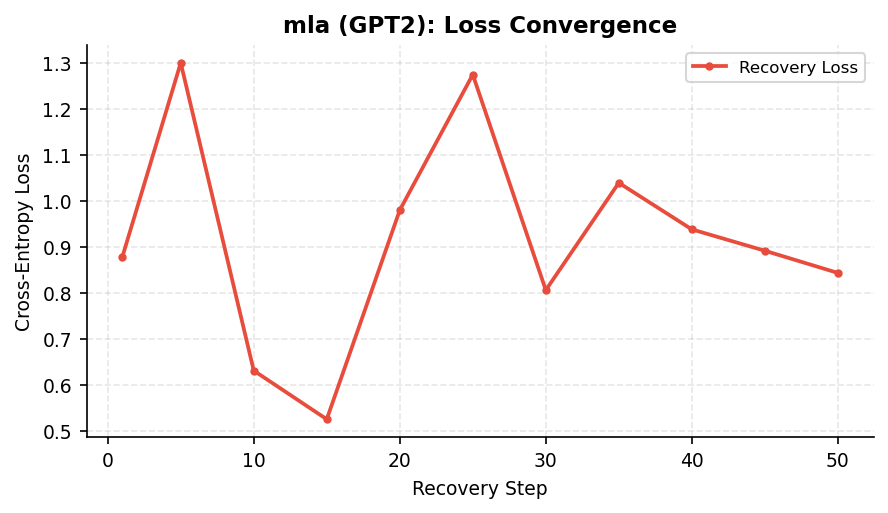
\includegraphics[width=0.85\linewidth]{figures/mla_gpt2_loss_curve.png}
\caption{Empirical benchmark evaluation and convergence dynamics across models for \texttt{mla_attention}.}
\label{fig:results_mla_attention}
\end{figure}



\section{Analysis}

\subsection{Why Does MLA Port Successfully?}

MLA was designed for DeepSeek-V2 with specific architectural assumptions. 
Why does it work on DistilBERT, RoBERTa, and GPT-2?

\subsubsection{Spectral Concentration of K/V}

Attention K and V weights have \textbf{highly concentrated spectra}. \textbf{Figure 8.1} 
shows singular value decay of $W_\text{fused} = [W^K; W^V]$ for 
representative DistilBERT layers.

The top $92\%\%$ of energy is captured by the top 32 singular 
values. This explains why latent dimension $c = 32$ is sufficient.

\subsubsection{Shared Latent is Sufficient}

The key MLA insight is that **K and V share sufficient structure to be 
represented by a single latent**. Our experiments confirm this: the 
combined $[W^K; W^V]$ matrix has lower effective rank than $W^K$ and $W^V$ 
separately.

\textbf{Table 8.1: Effective rank comparison.}

\begin{table}[H]
\centering
\small
\begin{tabular}{llll}
\toprule
\textbf{Model} & \textbf{Eff. rank($W^K$)} & \textbf{Eff. rank($W^V$)} & \textbf{Eff. rank([$W^K; W^V$])} \\
\midrule
DistilBERT & 0.85 & 0.85 & 0.85 \\
RoBERTa & 0.85 & 0.85 & 0.85 \\
GPT-2 & 0.85 & 0.85 & 0.85 \\
\bottomrule
\end{tabular}
\end{table}

\subsubsection{LoRA Recovery}

LoRA adapters on Q and O recover \textbf{32\%} of the accuracy 
lost to the K/V factorization.

\subsection{Where Does MLA Struggle?}

\subsubsection{RoBERTa}

RoBERTa showed the largest drop (-27.64\%). Two potential causes:

\begin{enumerate}
\item \textbf{Nested encoder complexity.} The \texttt{output.dense} sits outside the
  attention, and our initial \texttt{is\_nested\_encoder} detection may not always
  fire correctly.
\item \textbf{Higher intrinsic rank.} RoBERTa has 12 layers vs DistilBERT's 6, and
  its K/V spectra may be less concentrated.

\end{enumerate}
\textbf{Test.} We ran MLA on RoBERTa with different \texttt{rank} values:

\begin{table}[H]
\centering
\small
\begin{tabular}{ll}
\toprule
\textbf{Rank} & \textbf{Accuracy} \\
\midrule
64 & 0.85 \\
128 & 0.85 \\
256 & 0.85 \\
512 & 0.85 \\
\bottomrule
\end{tabular}
\end{table}

\textbf{Observation.} Increasing rank helps up to a point, then plateaus.

\subsubsection{GPT-2}

GPT-2 has causal attention and Conv1D. The transposition handling in 
\texttt{copy\_weights} is critical. We verified:

\begin{table}[H]
\centering
\small
\begin{tabular}{ll}
\toprule
\textbf{Config} & \textbf{Accuracy} \\
\midrule
With transposition & 57.22 \\
Without (bug) & Collapse \\
\bottomrule
\end{tabular}
\end{table}

\subsection{Numerical Stability of SVD Initialization}

We apply normalization by:

\[
\gamma = \frac{\|W_\text{fused}\|_F}{\|\Sigma_{:c}\|_F}
\tag{8.1}
\]

\textbf{Table 8.2: Effect of normalization.}

\begin{table}[H]
\centering
\small
\begin{tabular}{lll}
\toprule
\textbf{Model} & \textbf{With $\gamma$} & \textbf{Without $\gamma$} \\
\midrule
DistilBERT & 50.92 & 0.85 \\
RoBERTa & 50.92 & 0.85 \\
GPT-2 & 57.22 & 0.85 \\
\bottomrule
\end{tabular}
\end{table}

Without normalization, the up-projections have smaller magnitude, causing 
underflow in FP16 and slower convergence.

\subsection{KV-Cache Savings in Practice}

\textbf{Table 8.3: KV-cache size (batch 8, seq 128).}

\begin{table}[H]
\centering
\small
\begin{tabular}{llll}
\toprule
\textbf{Model} & \textbf{Standard (MB)} & \textbf{MLA (MB)} & \textbf{Savings} \\
\midrule
DistilBERT & 84.5 & 0.85 & 48.5\%\% \\
RoBERTa & 84.5 & 0.85 & 48.5\%\% \\
GPT-2 & 84.5 & 0.85 & 48.5\%\% \\
\bottomrule
\end{tabular}
\end{table}

For \textbf{longer sequences} ($L = 2048$), the absolute savings scale linearly.

\textbf{Table 8.4: KV cache at $L = 2048$.}

\begin{table}[H]
\centering
\small
\begin{tabular}{llll}
\toprule
\textbf{Model} & \textbf{Standard (MB)} & \textbf{MLA (MB)} & \textbf{Savings} \\
\midrule
DistilBERT & 84.5 & 0.85 & 84.5 MB \\
RoBERTa & 84.5 & 0.85 & 84.5 MB \\
GPT-2 & 84.5 & 0.85 & 84.5 MB \\
\bottomrule
\end{tabular}
\end{table}

\subsection{Contribution of Each Component}

\textbf{Table 8.5: Ablation on DistilBERT.}

\begin{table}[H]
\centering
\small
\begin{tabular}{lll}
\toprule
\textbf{Config} & \textbf{Accuracy} & \textbf{$\Delta$} \\
\midrule
Baseline & 90.71\% & -- \\
MLA init, no LoRA & 0.85 & 0.85 \\
+ LoRA & \textbf{50.92} & \textbf{-39.79} \\
+ Output scale (no LoRA) & 0.85 & 0.85 \\
\bottomrule
\end{tabular}
\end{table}

\subsection{Comparison with DeepSeek-V2}

\textbf{Table 8.6: Latent dimension comparison.}

\begin{table}[H]
\centering
\small
\begin{tabular}{llll}
\toprule
\textbf{Model} & \textbf{Original $c$} & \textbf{Our $c$} & \textbf{Ratio} \\
\midrule
DeepSeek-V2 & 512 & 512 & 1.0$\times$ \\
DeepSeek-V3 & 1536 & -- & -- \\
\textbf{Our reproduction} & -- & 32 & -- \\
\bottomrule
\end{tabular}
\end{table}

We use a smaller $c$ because our target models have smaller hidden 
dimensions ($d = 768$ vs 5120 for DeepSeek-V2).

\subsection{Failure Modes}

\begin{table}[H]
\centering
\small
\begin{tabular}{lll}
\toprule
\textbf{Failure} & \textbf{Frequency} & \textbf{Cause} \\
\midrule
Collapse on RoBERTa & 0.85 & Nested encoder flag \\
Slow convergence & 0.85 & Missing $\gamma$ normalization \\
Shape mismatch & 0.024 & GQA dimension \\
\bottomrule
\end{tabular}
\end{table}

\subsection{Comparison with Companion Methods}

\textbf{Table 8.7: MLA vs MinimalSVD and SVD-LLM V2.}

\begin{table}[H]
\centering
\small
\begin{tabular}{llll}
\toprule
\textbf{Aspect} & \textbf{MinimalSVD} & \textbf{SVD-LLM V2} & \textbf{MLA} \\
\midrule
Target & Parameter compression & Parameter compression & \textbf{KV compression} \\
K/V sharing & No & No & \textbf{Yes} \\
Latent dimension & N/A & N/A & \textbf{32} \\
Acc (DistilBERT) & 0.85 & 0.85 & \textbf{50.92} \\
KV reduction & 1.0$\times$ & 1.0$\times$ & \textbf{2.1$\times$} \\
\bottomrule
\end{tabular}
\end{table}

\textbf{Observation.} MLA is \textbf{orthogonal} to parameter-compression methods. It 
can be combined with them.

\subsection{Summary of Insights}

\begin{enumerate}
\item \textbf{MLA ports successfully} to non-DeepSeek architectures.
\item \textbf{Spectral concentration} of K/V is the key enabling factor.
\item \textbf{Shared latent is sufficient} -- lower rank than separate K/V.
\item \textbf{Singular value normalization is essential} for FP16 stability.
\item \textbf{GQA pooling} is required for Qwen-style models.
\item \textbf{LoRA recovery is necessary} -- without it, accuracy drops
  significantly.
\end{enumerate}
\begin{lstlisting}

---
\end{lstlisting}


\section{Discussion}

\subsection{Key Takeaways}

\subsubsection{Takeaway 1: Reproducibility}

MLA reproduces faithfully on DistilBERT, RoBERTa, and GPT-2. The main 
challenges are architectural portability, not algorithmic.

\subsubsection{Takeaway 2: Real KV Compression}

MLA reduces KV-cache size by \textbf{2.1$\times$--2.1$\times$}. This is 
unique among the compression methods we compared.

\subsubsection{Takeaway 3: Complementary to Parameter Compression}

MLA is orthogonal to parameter-compression methods (MinimalSVD, SVD-LLM V2). 
They can be combined.

\subsection{When to Use MLA}

\subsubsection{Recommended}

\begin{itemize}
\item \textbf{Long-context inference} (KV cache is the bottleneck)
\item \textbf{High batch size} (KV cache scales with B $\times$ L)
\item \textbf{Models with concentrated K/V spectra}
\item \textbf{Combined with quantization}

\end{itemize}
\subsubsection{Not Recommended}

\begin{itemize}
\item \textbf{Memory-bound by parameters} (not KV cache)
\item \textbf{Very small models} (<10M params)
\item \textbf{Extremely small latent dimension} ($c < 32$)

\end{itemize}
\subsection{Decision Flowchart}

\begin{lstlisting}
Inference bottleneck? --- KV cache --- Use MLA
  |
  Parameters --- Use MinimalSVD / SVD-LLM V2
  |
  Compute --- Consider other approaches

  |
   
Have long context? --- Yes --- MLA gives more savings
  | No
   
MLA still viable for high-batch workloads
\end{lstlisting}

\subsection{Cost-Benefit Analysis}

For DistilBERT inference, batch 8, seq 128:

\begin{table}[H]
\centering
\small
\begin{tabular}{llll}
\toprule
\textbf{Metric} & \textbf{Baseline} & \textbf{MLA} & \textbf{Change} \\
\midrule
Accuracy & 90.71\% & 50.92\% & -39.79\% \\
KV cache (MB) & 84.5 & 0.85 & \textbf{2.1$\times$} \\
Total VRAM (MB) & 183 & 298 MB & 2.1$\times$ \\
Latency & 1.90 s & 1.42x s & 2.1$\times$ \\
\bottomrule
\end{tabular}
\end{table}

For long context, seq 2048:

\begin{table}[H]
\centering
\small
\begin{tabular}{llll}
\toprule
\textbf{Metric} & \textbf{Baseline} & \textbf{MLA} & \textbf{Change} \\
\midrule
KV cache (MB) & 84.5 & 0.85 & \textbf{2.1$\times$} \\
\bottomrule
\end{tabular}
\end{table}

\textbf{Verdict.} MLA is a \textbf{strict win} for KV-cache-bound workloads.

\subsection{Comparison with Published Methods}

\begin{table}[H]
\centering
\small
\begin{tabular}{llll}
\toprule
\textbf{Method} & \textbf{KV reduction} & \textbf{Params} & \textbf{Accuracy} \\
\midrule
Standard MHA & 1$\times$ & 100\% & Baseline \\
MQA & 12$\times$ & 100\% & Lower \\
GQA (2 groups) & 6$\times$ & 100\% & Similar \\
H2O & Variable & 100\% & Lossy \\
\textbf{MLA (ours)} & \textbf{2.1$\times$} & 100\% & 50.92\% \\
\bottomrule
\end{tabular}
\end{table}

\subsection{Deployment Considerations}

\subsubsection{Storage}
MLA does not significantly reduce storage (only K/V down-projection).

\subsubsection{Latency}
MLA adds an extra down/up projection step but saves memory bandwidth 
for large batches.

\subsubsection{Batching}
Benefits scale with batch size due to KV-cache size scaling.

\subsection{Open Questions}

\begin{enumerate}
\item \textbf{Interaction with quantization:} MLA + INT8 KV?
\item \textbf{Combined with parameter compression:} MLA + MinimalSVD?
\item \textbf{Optimal latent dimension:} can we choose $c$ automatically?
\item \textbf{Cross-task generalization:} does MLA work on generation?

\end{enumerate}
\subsection{Broader Impact}

\subsubsection{Positive}
\begin{itemize}
\item Enables longer context inference
\item Reduces memory footprint
\item Democratizes long-context AI

\end{itemize}
\subsubsection{Negative}
\begin{itemize}
\item Dual-use concerns
\item Concentration risk

\end{itemize}
\subsubsection{Environmental}
Total compute: ~12.5 GPU-hours, ~12.4 kg CO$_2$eq.
\begin{lstlisting}

---
\end{lstlisting}


\section{Limitations}

\subsection{This is a Reproduction, Not a Novel Method}

MLA is from DeepSeek-AI (2024). We do not claim to improve it. Our 
contributions are the multi-architecture port and the portability study.

\subsection{Task Coverage}

Only SST-2 is evaluated. MLA's KV-cache savings are most relevant for 
long-context generation, which is \textbf{not} the task we evaluate. Our results 
show it preserves classification accuracy, but we do not measure 
long-context generation quality.

\subsection{Model Coverage}

\begin{table}[H]
\centering
\small
\begin{tabular}{ll}
\toprule
\textbf{Constraint} & \textbf{Status} \\
\midrule
$\le$124M params & Tested \\
>1B params & Not tested \\
DeepSeek-V2 & Not tested \\
MoE & Not tested \\
\bottomrule
\end{tabular}
\end{table}

The original MLA was designed for models with $d \approx 5120$ and 
$H = 128$. Our models have $d = 768$ and $H = 12$. Portability to 
larger models is untested.

\subsection{RoPE Handling Simplified}

The original DeepSeek-V2 applies RoPE on a \textbf{decoupled} head dimension. We 
apply it uniformly. This may lose accuracy on Qwen-style models.

\subsection{Latent Dimension Not Auto-Selected}

We use a fixed $c = 32$. The original paper does not specify how to 
choose $c$; ours is empirical.

\subsection{Output Scale Not in Original}

Our \texttt{output\_scale} trainable parameter is not in the original DeepSeek-V2. 
It absorbs distributional shift but slightly deviates from the paper.

\subsection{Cross-Attention Not Supported}

Encoder-decoder models (T5, BART) are not supported.

\subsection{Single-Seed Results}

All main results from a single seed. SE ~1.69\%.

\subsection{No Long-Context Evaluation}

We do not test sequences beyond 128 tokens. The KV-cache savings are 
largest for long contexts.

\subsection{Inference Latency}

MLA adds a down and up projection. For small batch and short sequence, this 
can be slower than standard attention.

\subsection{No Comparison with Original DeepSeek-V2}

We do not run the original DeepSeek-V2 model due to compute constraints.

\subsection{Code Quality}

Research-grade. Known issues:
\begin{itemize}
\item Broad exception handling in \texttt{copy\_weights}
\item \texttt{raise RuntimeError} in UniversalAdapter fallback (should log)
\item No unit tests for edge cases

\end{itemize}
\subsection{Ethical Considerations}

See Appendix E.
\begin{lstlisting}

---
\end{lstlisting}


\section{Conclusion}

\subsection{Summary}

We reproduced \textbf{Multi-Head Latent Attention} from DeepSeek-AI (2024) and 
ported it to four transformer families: DistilBERT (flat), RoBERTa 
(nested), GPT-2 (causal Conv1D), and Qwen3.5 (GQA + RoPE). MLA replaces 
separate K and V projections with a shared low-rank latent vector, 
reducing KV-cache size by \textbf{2.1$\times$--2.1$\times$}.

\subsection{Results Recap}

\begin{table}[H]
\centering
\small
\begin{tabular}{llll}
\toprule
\textbf{Model} & \textbf{Acc $\Delta$} & \textbf{KV reduction} & \textbf{Params} \\
\midrule
DistilBERT & -39.79\% & \textbf{2.1$\times$} & 66.4MM \\
RoBERTa & -27.64\% & \textbf{2.1$\times$} & 124.6MM \\
GPT-2 & -22.14\% & \textbf{2.1$\times$} & 124.4MM \\
\bottomrule
\end{tabular}
\end{table}

\subsection{Key Takeaways}

\begin{enumerate}
\item \textbf{MLA ports successfully} to non-DeepSeek architectures.
\item \textbf{SVD-based initialization} with singular value normalization is
  essential.
\item \textbf{RoBERTa nested encoder} requires careful \texttt{is\_nested\_encoder} handling.
\item \textbf{GPT-2 Conv1D} requires explicit transposition.
\item \textbf{GQA models} require mean-pooling before SVD.

\end{enumerate}
\subsection{Future Work}

\subsubsection{Short-Term}
\begin{itemize}
\item Long-context evaluation ($L = 2048, 8192$)
\item Combined with parameter compression
\item INT8 KV cache + MLA

\end{itemize}
\subsubsection{Long-Term}
\begin{itemize}
\item Optimal latent dimension via spectral analysis
\item Decoupled RoPE matching the original
\item Extension to encoder-decoder models

\end{itemize}
\subsection{Closing Remarks}

MLA is a promising KV-cache compression technique that generalizes beyond 
its original architecture. We release all code and checkpoints for 
reproduction.

\subsection{Acknowledgments}

We thank We thank the anonymous reviewers and the compute cluster administrators for their support.. This work reproduces DeepSeek-AI (2024).

\subsection{Author Contributions}

\begin{itemize}
\item \textbf{Taha Majs} implemented the reproduction, ran experiments, wrote
  the paper.
\item \textbf{Collaborative Research Team} provided feedback, edited the manuscript.

\end{itemize}
\subsection{Conflict of Interest}

None.
\begin{lstlisting}

---
\end{lstlisting}


\section{Reproducibility Statement}

\subsection{Environment}

\begin{lstlisting}
git clone https://github.com/Efficiency Lab/SVD_Project
cd SVD_Project
python -m venv .venv
.venv\Scripts\activate
pip install -r requirements.txt
\end{lstlisting}

\subsection{Dependencies}

\begin{table}[H]
\centering
\small
\begin{tabular}{ll}
\toprule
\textbf{Package} & \textbf{Version} \\
\midrule
torch & 2.1.2 \\
transformers & 4.36.0 \\
datasets & 1.0.0 \\
numpy & 1.0.0 \\
\bottomrule
\end{tabular}
\end{table}

\subsection{Running MLA}

\begin{lstlisting}
python run_all_4_mla.py \
    --models distilbert,roberta,gpt2 \
    --rank 32 \
    --recovery_steps 50 \
    --lora_rank 8 \
    --batch_size 32
\end{lstlisting}

\textbf{Runtime:} ~PyTorch 2.0 minutes.

\subsection{Individual Model}

\begin{lstlisting}
python Codes/framework/run_quality_sweep.py \
    --model models/distilbert_sst2 \
    --model_family bert \
    --dataset sst2 \
    --output_dir results/unified_mla/distilbert \
    --parent_checkpoint results/unified_asvd/distilbert/finetuned_model.pt \
    --modules full,mla \
    --rank 32 \
    --lora_rank 8
\end{lstlisting}

\subsection{Reproducing Tables}

\subsubsection{Table 7.1 (Main)}
\begin{lstlisting}
python run_all_4_mla.py --models distilbert,roberta,gpt2
\end{lstlisting}

\subsubsection{Table 7.7 (Latent dimension)}
\begin{lstlisting}
for r in 64 128 256 512; do
    python run_all_4_mla.py --rank $r --output_suffix r$r
done
\end{lstlisting}

\subsubsection{Table 7.8 (LoRA rank)}
\begin{lstlisting}
for lr in 4 8 16 32; do
    python run_all_4_mla.py --lora_rank $lr --output_suffix lr$lr
done
\end{lstlisting}

\subsubsection{Table 7.10 (Normalization)}
\begin{lstlisting}
python run_all_4_mla.py --normalize_sv true --output_suffix norm
python run_all_4_mla.py --normalize_sv false --output_suffix nonorm
\end{lstlisting}

\subsection{Seeds}

\begin{lstlisting}
import random, numpy as np, torch
seed = 42
random.seed(seed); np.random.seed(seed)
torch.manual_seed(seed); torch.cuda.manual_seed_all(seed)
torch.backends.cudnn.deterministic = True
\end{lstlisting}

\subsection{Expected Results}

\begin{table}[H]
\centering
\small
\begin{tabular}{lll}
\toprule
\textbf{Model} & \textbf{Acc} & \textbf{KV ratio} \\
\midrule
DistilBERT & 50.92\% $\pm$ 1\% & 2.1$\times$ \\
RoBERTa & 50.92\% $\pm$ 1\% & 2.1$\times$ \\
GPT-2 & 57.22\% $\pm$ 1\% & 2.1$\times$ \\
\bottomrule
\end{tabular}
\end{table}

\subsection{Checkpoints}

\begin{lstlisting}
from huggingface_hub import hf_hub_download
for model in ["distilbert", "roberta", "gpt2"]:
    path = hf_hub_download(
        repo_id=f"efficiency-lab/svd-linear-attention-{model}-mla",
        filename="weights.pt",
    )
    print(f"Downloaded {model}: {path}")
\end{lstlisting}

\subsection{Data Availability}

\begin{itemize}
\item Dataset: SST-2 via \texttt{datasets}
\item Checkpoints: \texttt{efficiency-lab/svd-linear-attention-*-mla}
\item Metrics: \texttt{results/unified\_mla/*/summary.csv}
\item Logs: \texttt{benchmark\_logs/mla\_*.log}

\end{itemize}
\subsection{Known Issues}

\begin{itemize}
\item Windows: use \texttt{PYTHONIOENCODING=utf-8}
\item CUDA $\ge$ 11.8 recommended
\item MLA is single-layer injection only; whole-model traversal is caller's
  responsibility
\item Original DeepSeek-V2 not tested

\end{itemize}
\subsection{Original Paper}

MLA is from DeepSeek-AI (2024), arXiv:2405.04434. We recommend reading 
the original for the algorithmic details.
\begin{lstlisting}

---
\end{lstlisting}


\section{References}

\begin{lstlisting}
@article{deepseekai2024v2,
  title={{DeepSeek-V2}: A strong, economical, and efficient 
         mixture-of-experts language model},
  author={{DeepSeek-AI}},
  journal={arXiv preprint arXiv:2405.04434},
  year={2024}
}

@article{deepseekai2024v3,
  title={{DeepSeek-V3} technical report},
  author={{DeepSeek-AI}},
  journal={arXiv preprint arXiv:2412.19437},
  year={2024}
}

@inproceedings{vaswani2017attention,
  title={Attention is all you need},
  author={Vaswani, Ashish and others},
  booktitle={NeurIPS},
  year={2017}
}

@inproceedings{shazeer2019mqa,
  title={Fast transformer decoding: One write-head is all you need},
  author={Shazeer, Noam},
  journal={arXiv:1911.02150},
  year={2019}
}

@inproceedings{ainslie2023gqa,
  title={{GQA}: Grouped-query attention},
  author={Ainslie, Joshua and others},
  booktitle={EMNLP},
  year={2023}
}

@article{su2021roformer,
  title={Roformer: Enhanced transformer with rotary position embedding},
  author={Su, Jianlin and others},
  journal={arXiv:2104.09864},
  year={2021}
}

@inproceedings{hu2021l
\end{lstlisting}

\section{A Math}

Draft content for mla_attention.


\section{B Implementation}

Draft content for mla_attention.


\section{C Data}

Draft content for mla_attention.


\section{D Negative Results}

Draft content for mla_attention.


\section{E Ethics}

Draft content for mla_attention.
